\begin{appendices}
	\section{\ep - Number of tracks in data and Monte Carlo simulation}\label{app:a}
	
	\begin{figure}[H]
		\centering
		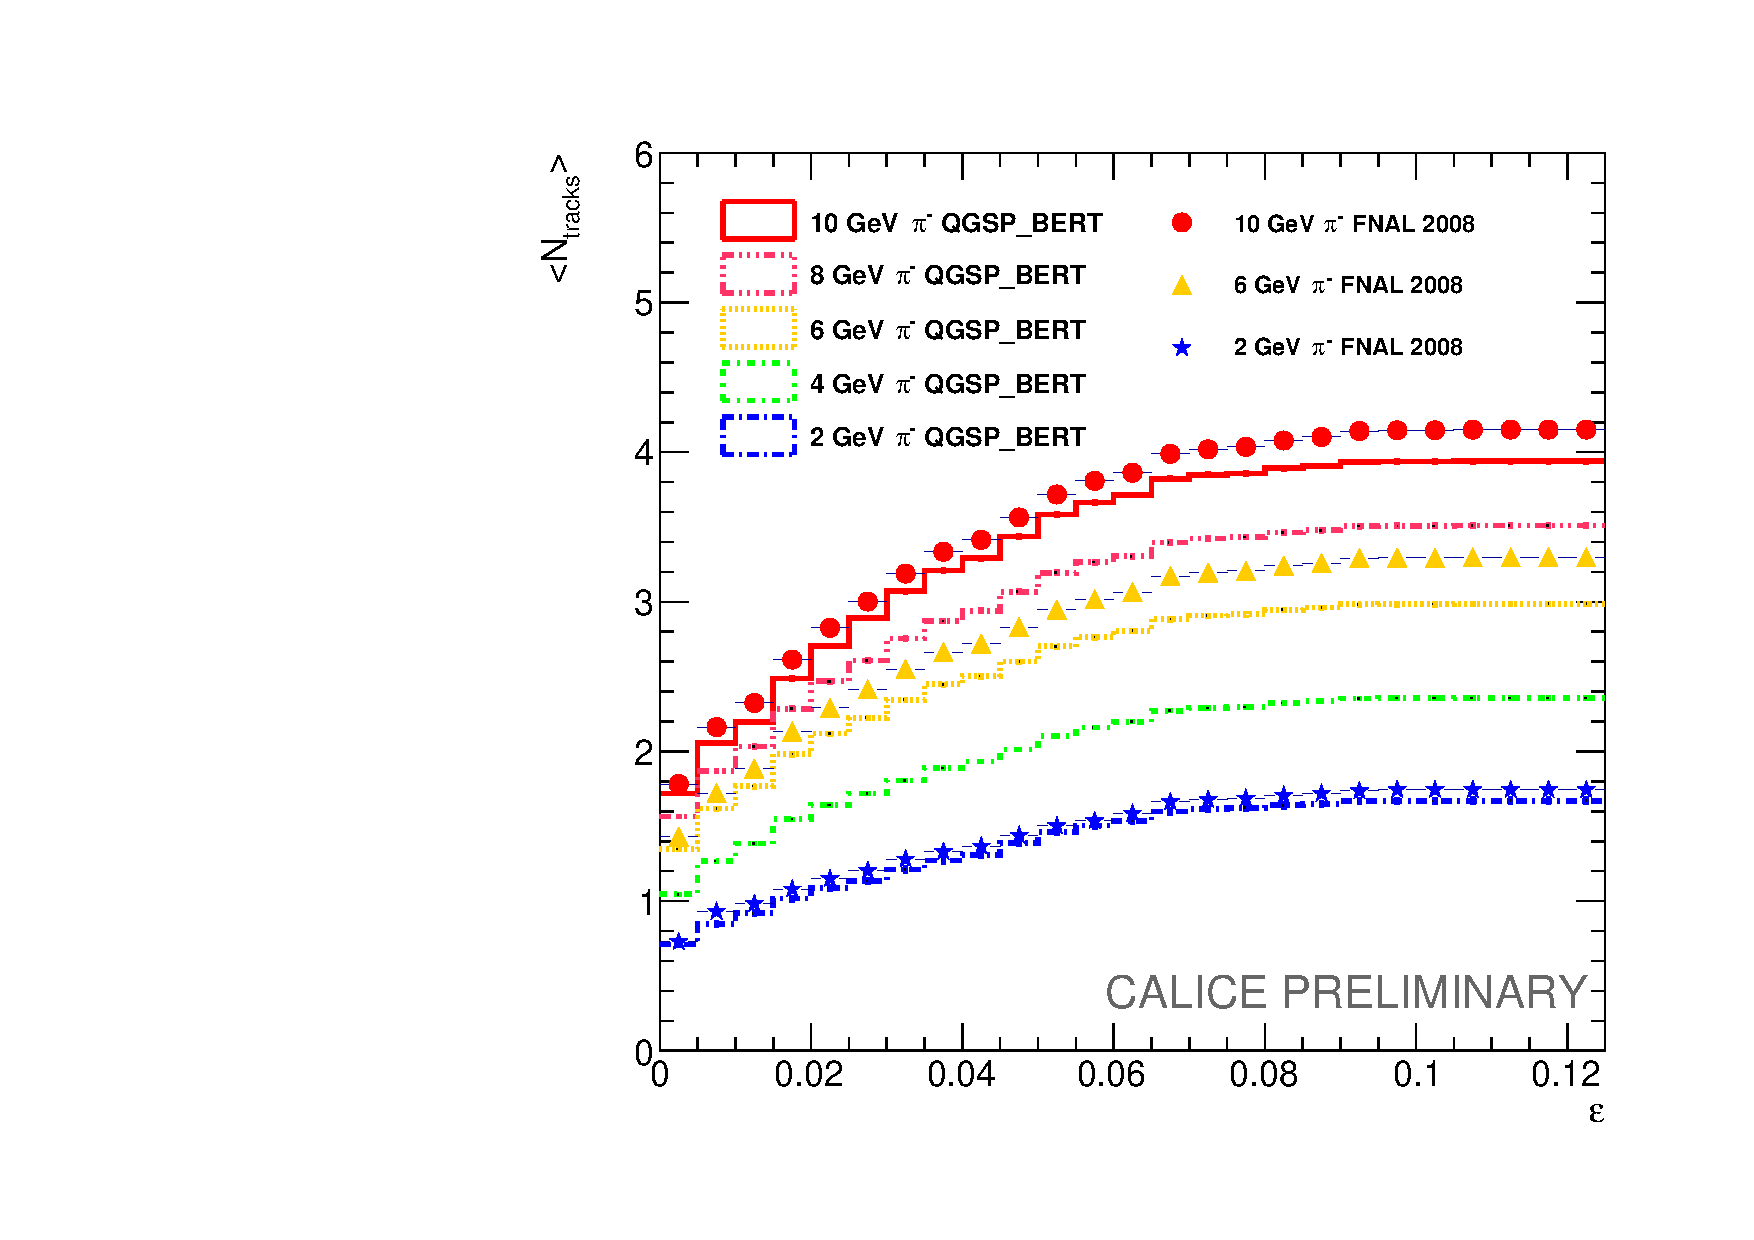
\includegraphics[width=0.5\textwidth]{ECAL/plots/combination.pdf}
		\caption{\label{fig:epsilonsysdata} \sl Mean number of tracks found by the \tfa\ as a function of $\varepsilon$ values for 2, 4, 6, 8 and 10\,GeV beam energy for data (bullets) and for \qgsp\ physics list simulation (lines). Events without a detected interaction region are excluded.}
	\end{figure}
	
	For future reference the Fig. \ref{fig:epsilonsysdata} shows a comparison between data and Monte Carlo for the studies presented in Sec.~\ref{sec:systematics}. 
	
	\section{Polar angle and track length as a function of the \ep}\label{app:b}
	
	Figure \ref{fig:thetaepsilonsys} presents the variation of $\left<\theta\right>$ in \qgsp\ simulation  for different beam energies as a function of the \ep\ value. 
	The mean polar angle saturates for large $\varepsilon$. The empirically chosen value of $\varepsilon=0.03$ is close to a local minimum of the function, therefore, the $<\theta>$ observable is stable against a small variation of the $\varepsilon$ value. 
	
	The mean track length $<l>$ as function of $\varepsilon$ for different beam energies is shown in Fig. \ref{fig:lepsilonsys}. 
	The function has a local maximum around $\varepsilon=0.03$ and it saturates for large $\varepsilon$. 
	These observations can be explained as follows:
	\begin{itemize}
		\item At $\varepsilon \to 0$ only small pencil-like clusters are considered as tracks. The small tracks can fit the \ecal\ pad volume for any direction. Therefore, $<\theta>$ is large; 
		\item If the $\varepsilon$ value is slightly above zero, the longer clusters, with some amount of adjacent hits become tracks. These tracks have smaller $<\theta>$ angle due to a fact that the \ecalp\ has 30 layers in depth and 18 $\times$ 18 lateral size.  
		\item With large $\varepsilon$ values also spherical shaped clusters are accepted as tracks. These clusters have a small amount of hits, since otherwise, they would be counted as an interaction region. The algorithm can assign any direction for these spherical clusters, resulting in an increase of $\left<\theta\right>$ and a decrease of the mean track length. 
	\end{itemize}
	
	
	
	\begin{figure}[H]
		\centering
		\begin{subfigure}{0.5\textwidth}
			\centering
			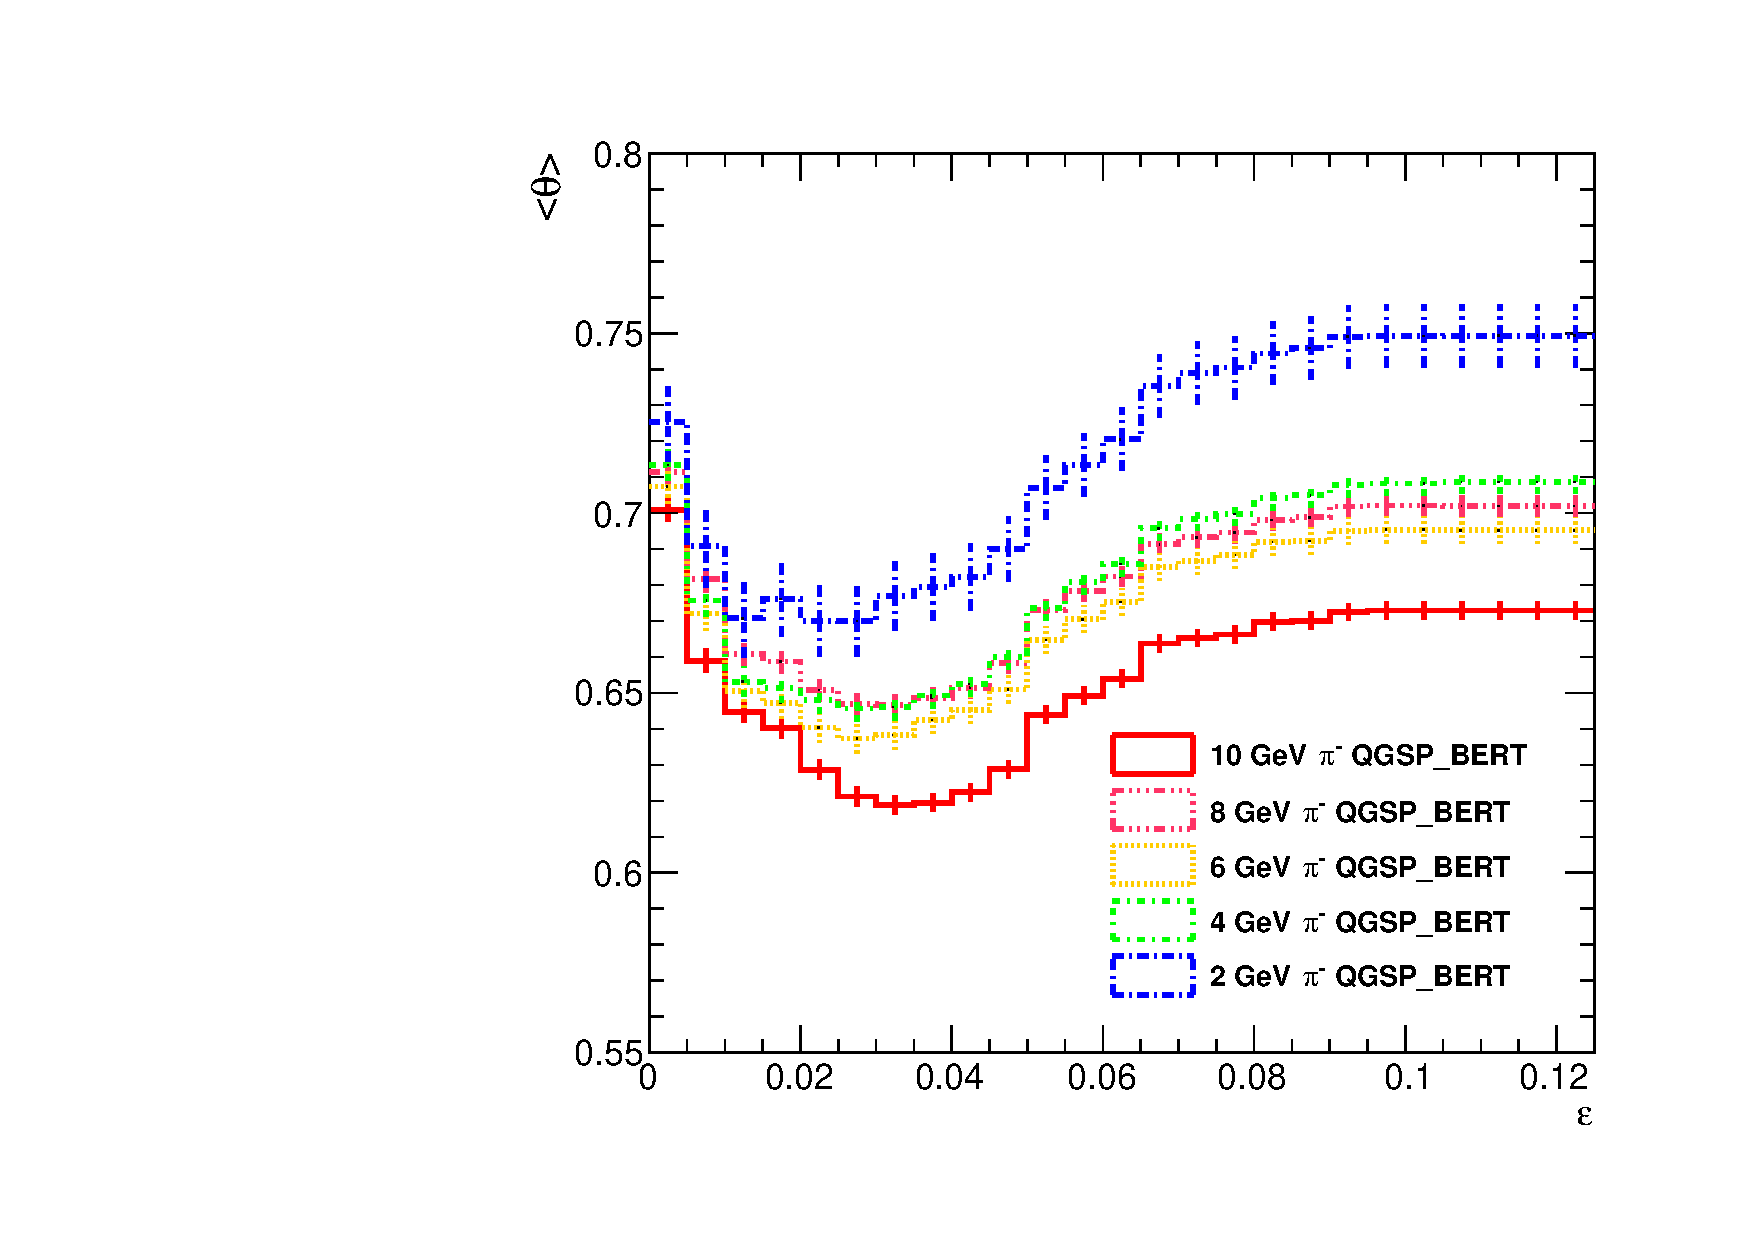
\includegraphics[width=.90\linewidth]{ECAL/plots/sys-theta.pdf}
			\caption{\label{fig:thetaepsilonsys} }
		\end{subfigure}% 
		\begin{subfigure}{0.5\textwidth}
			\centering
			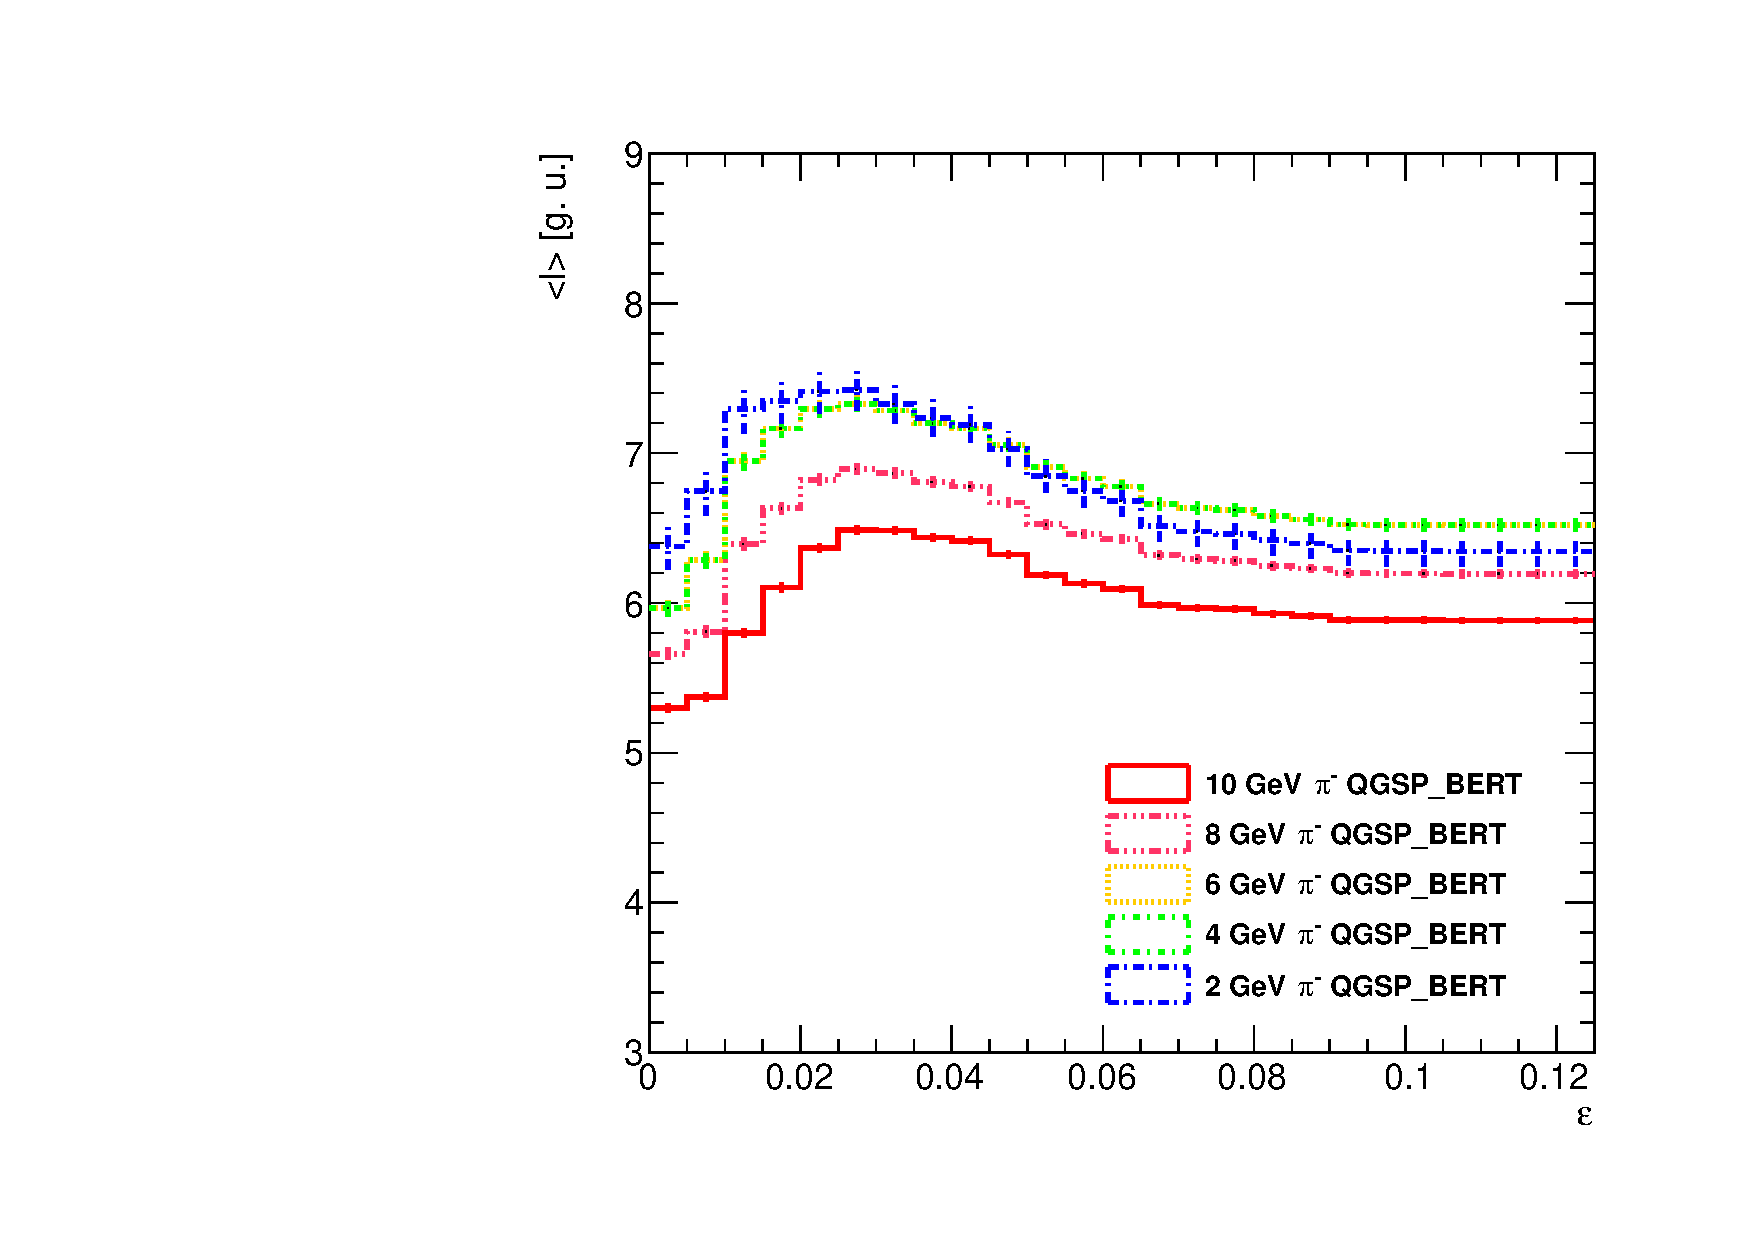
\includegraphics[width=.90\linewidth]{ECAL/plots/sys-l.pdf}
			\caption{\label{fig:lepsilonsys} }
		\end{subfigure}
		\caption{\label{fig:syslthetaexample} \sl Mean $\theta$ angle (a) and mean track length $l$ (b) of the tracks found by the \tfa\ with different \ep\ values for 2, 4, 6, 8 and 10\,GeV beam energy in \qgsp\ simulation. The minimum value of $\left<\theta\right>$ and the maximum value of the track length is around the empirically chosen value of $0.03$. }
	\end{figure}
	
\end{appendices}
%The following plots in Fig. \ref{fig:rtotexample} and \ref{fig:rtotalrgraph} allow to establish a connection between Ref. \cite{bib:Naomi} and the present study. Regarding the difference in units of measurement and different selection by interaction layer, the Fig. \ref{fig:rtotalrgraph} is similar to its analogue in Ref. \cite{bib:Naomi}.
%\begin{figure}[H]
%\centering
%\begin{subfigure}{0.5\textwidth}
%\centering
%\includegraphics[width=.90\linewidth]{ECAL/plots/r-total-2.pdf}
%\caption{\label{fig:rtot2} 2\,GeV primary particle.}
%\end{subfigure}% 
%\begin{subfigure}{0.5\textwidth}
%\centering
%\includegraphics[width=.90\linewidth]{ECAL/plots/r-total-10.pdf}
%\caption{\label{fig:rtot10} 10\,GeV primary particle.}
%\end{subfigure}
%\caption{\label{fig:rtotexample} A comparison of mean radius of event hits between Monte Carlo samples and data with 2 (left) and 10 (right) GeV beam energy. The histograms are normalized to unity in order to compare samples with different event number. Error bars on the plot represent statistical uncertainties only.}
%\end{figure}

%\begin{figure}[H]
%\centering
%\includegraphics[width=0.5\textwidth]{ECAL/plots/r-total-graph.pdf}
%\caption{\label{fig:rtotalrgraph} A mean radius of hits in the \ecal\ for data and various Monte Carlo physics lists as a function of beam energy (2\,GeV to 10\,GeV). Error regions on the graph represent statistical uncertainties only.}
%\end{figure}

%\begin{figure}[H]
%\centering
%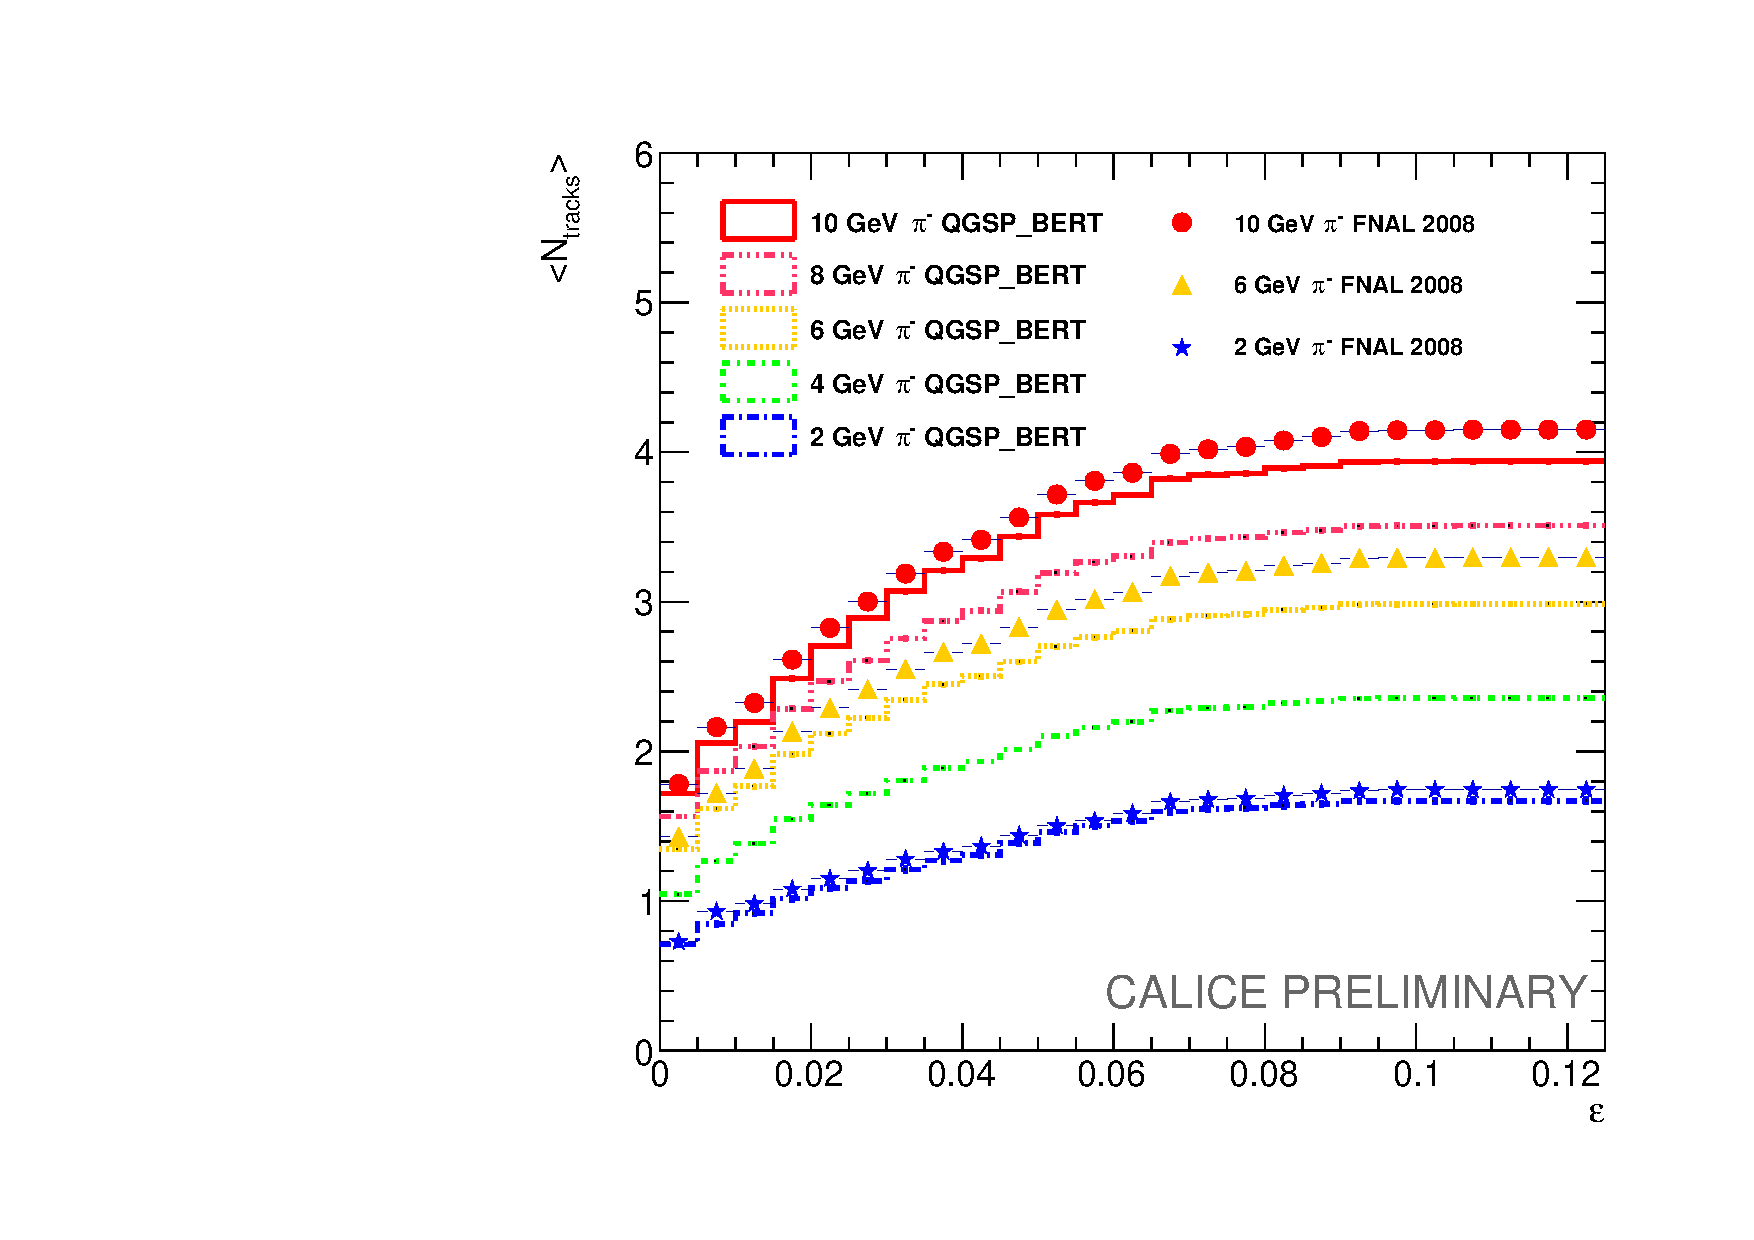
\includegraphics[width=0.5\textwidth]{ECAL/plots/combination.pdf}
%\caption{\label{fig:epsilondatasys} Mean number of tracks found by the \tfa\ with different \ep\ values for 2, 4, 6, 8 and 10\,GeV beam energy of the \qgsp\ simulation and data. The difference between data and corresponding simulation curves is caused by an underestimation of number of clusters by the physics list model. The saturation value of $<N_{tracks}>$ is gradually increasing with the beam energy. }
%\end{figure}

